\documentclass[12pt]{article}

% set margins and spacing
\addtolength{\textwidth}{1.3in}
\addtolength{\oddsidemargin}{-.65in} %left margin
\addtolength{\evensidemargin}{-.65in}
\setlength{\textheight}{9in}
\setlength{\topmargin}{-.5in}
\setlength{\headheight}{0.0in}
\setlength{\footskip}{.375in}
\renewcommand{\baselinestretch}{1.0}
\linespread{1.0}



% load miscellaneous packages
\usepackage{csquotes}
\usepackage[american]{babel}
\usepackage[usenames,dvipsnames]{color}
\usepackage{graphicx,amsbsy,amssymb, amsmath, amsthm, MnSymbol,bbding,times, verbatim,bm,pifont,pdfsync,setspace,natbib}
\usepackage{natbib}
\usepackage{datetime}
\usepackage{xcolor}
\usepackage[normalem]{ulem}
\usepackage{appendix}
\usepackage{setspace}
\usepackage{nameref}


% enable hyperlinks and table of contents
\usepackage[pdftex,
bookmarks=true,
bookmarksnumbered=false,
pdfview=fitH,
bookmarksopen=true,hyperfootnotes=false]{hyperref}

% define environments
\newtheorem{definition}{Definition}
\newtheorem{fact}{Fact}
\newtheorem{result}{Result}
\newtheorem{proposition}{Proposition}




\begin{document}
\title{Nepobabies: Labor Market Entry and Nepotistic Behavior of Young Adults}
\author{Rachel Rabinowitz\thanks{Syracuse University, Maxwell School of Citizenship and Public Affairs. Email: rhrabino@syr.edu.} \and Ryan Seely\thanks{Syracuse University, Maxwell School of Citizenship and Public Affairs. Email: rpseely@syr.edu. 
We would like to thank Professor Kristy Buzard and Dylan Eldred for their guidance and support. We also thank Professor Maria Zhu for her work on this project that gave us this opportunity.}}
\date{\vskip-.1in \today}
\maketitle

\vskip.2in
\begin{center} {\bf Abstract} \end{center}

\begin{quote}
{\small We examine the effects of young adults entering the workforce during competitive labor markets and whether those seeking jobs during high unemployment times will be more likely to be in their parents' occupations. We create a framework where young adults working in the same industries as their parents are defined as products of nepotism and examine how trends of such nepotistic relationships behave under varying economic conditions. Our analysis uses chi-square tests of association, a logistic regression model, and a test of correlation to examine the differences in rates of nepotism for varying levels of unemployment. Using data from the General Social Survey (GSS) on young adults hired between 1960 and 2018, we find no greater likelihood of gaining employment within the same industry as ones parents during tighter labor markets, i.e., higher unemployment. We then use two-sample t-tests and chi-square tests to examine demographic trends of nepobabies. The significant findings are that nepotistic relationships are found in much greater frequency between parents and children of the same sex and that nepobabies feel that they have greater job security. }
\end{quote}


\bigskip
\section{Introduction} \label{sec:introduction}
"Nepobaby" is a term commonly used to describe nepotism among families, specifically among children of celebrities. The term is mostly used as an insulting phrase to imply someone's success was unearned and undeserving as they have had disproportionate access to job opportunities through their connections. This popular term, which is now used to describe the general population, extends to those gaining employment through familial connections in industries. Within our study, we define nepobabies as respondents who work in the same industry as at least one of their parents.

Our study examines whether nepobabies are more likely to be hired in competitive labor markets. By matching monthly unemployment rates to the estimated month in which someone was hired, we examine the relationship between the level of labor market competition and the likelihood of having a nepotistic industry relationship with a parent.
As documented by \cite{kahn_long-term_2010}, during times of competitive labor market conditions, young adults attempting to enter the workforce experience many difficulties and experience long term effects of entering a competitive labor market. These young adults struggling to enter into the workforce may turn to their connections to seek employment. As young professionals gain employment through relatives, nepobabies appear in the overall working population. This struggle for young professionals will incentivize them to use all of their resources to find a job. Therefore, we predicted that there will be more graduates joining their parent’s occupations under more competitive labor market conditions. 

Using data from the General Social Survey (GSS) and the Federal Reserve Economic Data (FRED), we analyze the relationship between labor market conditions and prevalence of nepobabies. Through chi-square analyses and a logistic regression model, we fail to gather enough evidence to reject our null hypothesis that there is no relationship between nepotism rates and the level of labor market competition. Nepobabies were not found to have been hired during higher unemployment times at a significantly higher rate than during less challenging economic times. Dividing our sample into  quartiles based on unemployment rates, we find no notable discrepancy between the rates of nepobabies hired in low versus high unemployment. We posit that this lack of significant difference in rates of nepotistic relationships over varying levels of labor market competition is due to strong desires to make use of parental resources for job finding purposes at all times, not just highly competitive ones. However, we do find that there is a small, but statistically significant, correlation (r = 0.0979) between the ratio of nepobabies to all workers hired at varying unemployment rates. Through a chi-square test, nepobabies were also found to be more likely to follow into the same profession as their parent of the same gender. Daughters were more likely to follow into their mother's profession and sons were more likely to follow into their father's. Through further testing on other characteristics in our sample, nepobabies feel greater job security within their workplaces.


\section{Literature Review} \label{sec:literature}
In recent decades, there have been many studies on relationships between parents and their children, the outlook of entering the workforce in tough economics times, and using social ties to gain employment. Within the workforce, the effects of entering the job market during tough economic times have been thoroughly analyzed. \cite{kahn_long-term_2010} describes the relationship between graduating in tough economic conditions and one's ability to find employment within the first two decades after graduation. By graduating in a worse-off economy, recent graduates should be expected to experience higher unemployment resulting in a greater likelihood of job mismatching. Job mismatching, a situation in which workers are forced into specific jobs that do not correspond with their education level or qualifications have resulted in many being pushed to seek higher education, hoping to both increase their human capital and to enter the workforce during better economic times. \cite{schwandt_unlucky_2019} and \cite{oreopoulos_short-_2012} describe the increasing likelihood to seek higher education during recessions or poor economic periods. The fewer job openings in a competitive labor market will be more attainable for higher-skilled workers, limiting the ability for recent graduates to find work after graduation. As a result, recent graduates entering the workforce may feel compelled to increase their human capital. The ability to differentiate oneself after graduation is a helpful tool in order to gain employment, especially in tight labor markets. This process of distinguishing oneself, attained through higher education, results in those more likely to move quickly throughout firms as they are in higher-demand than others. These highly-skilled individuals  may also be increasingly more likely to seek employment within lower-skilled jobs as they have much more variation within firms. These behaviors demonstrate how young workers entering the labor market are encouraged to do what they can to secure employment during tougher economic times, and why they might rely more on their parents, too.

Specifically within family units, \cite{kramarz_when_2014} discuss how important strong family ties are when seeking stable employment. As employees are more likely to disseminate information about job openings to their strong ties first due to stable networks and greater maintenance, those having close relationships with high-skilled individuals hear about job openings first. Firms also have become increasingly dependent on recruiting from social ties. The social connections of high-quality incumbent workers have become increasingly popular as firms believe these connections will exhibit the same qualities, especially when ex-ante information about the applicant is poor. Additionally, as described by both \cite{kramarz_when_2014} and \cite{hellerstein_dads_2011}, firms benefit from recruiting children of incumbent employees. \cite{hellerstein_dads_2011} describes women as particularly risk-adverse to explain why they may follow into their parents' professions, specifically their father’s occupation to prevent the risk of being jobless after their graduation. This finding, of young adults with a risk-averse quality following into a parent's profession, provides evidence for why nepotistic parent-child relations are formed and why they are common, and why we hypothesized that nepobabies would be more prevalent during higher unemployment times. Our finding, that approximately ten percent of all young adult workers surveyed are defined as nepobabies, demonstrates that a large portion of the workforce utilizes their familial relationships to establish careers and does provide evidence of this potentially risk-averse behavior.

There is also evidence that would support our null hypothesis, that rates of nepotism do not vary over the business cycle because the motivation to utilize parents as resources for job finding is already quite strong. \cite{kramarz2006nepotism} find that it is common for firms to hire the children of their employees, especially when the incumbent parent employee has higher status (salary and length of employment) and when the referred child employee is a less competitive hire than their classmates. Their research also speaks to the impetus of firms to hire referral employees, as firms that hire through referrals expectedly earn more than firms that hire through the market. Social psychologists \cite{vanhooft_nepotism_2011} document the psychological literature on the strong impact that parents have on their children's career choice simply by serving as an example. They note that parents can offer support to their children in terms of choosing a career, and such support was commonly offered for the parent's career. Such social influences on children in terms of choosing a career path may isolate the child's career choice from the effects of the economic conditions at which they enter the labor market.

There is little research that discusses both the impact of entering into competitive labor markets and the likelihood of using parents as social ties to gain employment. As discussed in previous economic literature, young adult children rely deeply on their relationships to gain employment, but few discuss the relationship between children’s reliance on their ties during poor economic conditions.


\section{Data}
\label{sec:data}
We use data collected from the GSS in the years 2002, 2006, 2010, 2014, and 2018. The surveys are largely conducted through 90-minute in-person interviews with English and Spanish-speaking adults to create a nationally representative sample. Only observations from the aforementioned years were analyzed due to the presence of a key variable (job length), which measures the approximate number of years a respondent has occupied their current job, and variables marking respondent and parent industries, being present in these five survey years. 

Using the job length variable and the GSS interview date variable, we estimated the month and year that a respondent was hired. The estimated month of hire was created by taking the interview date and subtracting the number of years of employment at the respondent's current job times 12. This means that the estimated month of hire is always the same month as the month a respondent was interviewed (unless a respondent had been employed for less than one year). This is due to the responses to the job length question only counted in one quarter of a year, three quarters of a year, and then years in counting numbers starting from one. This estimation of when respondents were hired allows us to group respondents based on the labor market they were hired in. Because the way that we estimate the labor market conditions at time of hiring is imprecise, we perform a sensitivity analysis that is discussed further in the results section.

Using the respondent’s age and estimated job length, we were able to limit our sample to those hired as young adults, which we defined as those hired younger than 30 years old. After limiting our sample to young adults, there were 2,852  observations of young adults and 287 young adult nepobabies. We defined nepobabies as having a matching industry code with at least one parent based on the 2007 North American Industry Classification System (NAICS) codes. Focusing on the population of those hired as young adults is ideal for examining nepotistic behavior because nepotistic relationships are more likely to be found from those hired as young adults. To determine a cutoff age for what we define as a "young adult," we used a logistic regression model, where hiring age is a predictor of nepobaby status. There is a 3.3 percent decrease in the likelihood of being a nepobaby associated with being hired each year older. Likewise, a chi-square analysis, testing the association between nepobaby status and age of hiring as 29 and younger or 30 and older shows a significant association at a 99.9 significance level. This age cutoff keeps the assumption of entering the job market and looking to parents for support as reasonable while simultaneously keeping the number of observations as high as possible.

The GSS data set, however, does not include data on unemployment rates at the time a respondent was interviewed or hired. Therefore, we use a monthly unemployment rate time series from the FRED. Using the FRED data merged with the GSS data set, we were able to assign an unemployment rate for the estimated month at which a respondent was hired. The monthly unemployment rate data spanned every month from January of 1960 to December of 2022 to include the range of all possible months a respondent in our data set was hired. For more detail on how all data was obtained and manipulated and how the data was merged and analyzed, review the information in the \nameref{sec:appendix}.


\section{Results}
\label{sec:result}

In the first part of our analysis, we use our data to determine whether nepotistic behavior changes significantly when labor markets become more competitive. In the second part, we analyze the demographics and parental relationships of nepobabies.

We created four groups of nepobabies: hired during low unemployment, hired during mid-low unemployment, hired during mid-high unemployment, and hired during high unemployment. In our analysis, low unemployment is considered to be an unemployment rate of less than or equal to 4.7 percent. Mid-low unemployment is considered to be greater than 4.7 percent but less than or equal to 5.5 percent. Mid-high unemployment is considered to be between 5.5 percent and 6.8 percent unemployment. High unemployment is considered to be greater than or equal to 6.8 percent. We determined these to be the cutoffs for the varying levels of unemployment rates because they represent the values marking each of the quartiles of all unemployment rates in our sample of hire months. By creating these four groups based on the quartiles, we create groups that are of roughly equal sizes of all respondents and optimal for testing our hypothesis.

\begin{table}[ht]
\centering
\begin{tabular}{l|cc|c}
 & Nepobabies & All Workers & Proportion \\ 
\hline 
Low & 71 & 807 & 0.0879 \\
Mid-low & 68 & 673 & 0.1019 \\
Mid-high & 67 & 652 & 0.1028 \\
High & 81 & 720 & 0.1125 \\
\hline 
No. Observations & 287 & 2846 & 0.1008 \\
\end{tabular}
\caption{Nepotism Counts and Ratios at Levels of Unemployment}
\label{tab:mytable}
\end{table}

We decided to use a chi-square test to determine if there is a statistically significant association between the categories of nepobaby status and unemployment level hire group. If there is a statistically significant association between the ratio of nepobabies in each group as we have defined them, then that provides evidence for our hypothesis that a greater level of labor market competition will produce a greater proportion of nepotism hires. It is important to note here that we cannot determine the actual level of nepotism per se, rather it is a measurement of the level of young adults joining the same industry as their parents. However, it is safe to assume that there is a positive association between the two levels.

After categorizing our sample of nepobabies into quartiles, we conducted a chi-square test measuring the association of nepotism status and the quartile level of unemployment at the time a worker was hired. Our null hypothesis is that there is no significant association between nepobaby status and unemployment level at hiring. The results of the chi-square test do not provide enough evidence to reject our null hypothesis with a p-value of 0.461 with three degrees of freedom. This test does not provide any evidence that there is an association between unemployment level at time of hiring and nepotism status. At this point, our null hypothesis stands. The ratios displayed in Figure 1 suggest that greater labor market competition does not compel young adults to utilize the resource that is their parents to find employment at significantly greater rates. However, from Figure 1, it does appear that below average competition might  remove the impetus for young adults to utilize that resource at a significantly different rate. To test this hypothesis, we ran two additional chi-square tests. In the first, we set up two unemployment level groups: the same low unemployment level group (less than or equal to 4.7 percent) and another group for all unemployment levels greater than 4.7 percent and tested the association between unemployment level and nepotism status. The p-value for this test was 0.152. For the second test, we tested the association between nepotism status and the low (less than or equal to 4.7 percent) and high (greater than or equal to 6.8 percent) unemployment level groups. The p-value for this test was 0.11. While these two results do not provide enough evidence, at conventional levels, to support the idea that lower unemployment levels remove the motivation for young adults to seek employment through their parental ties, it is worth noting that they are close to significant levels.

\begin{figure}
    \centering
    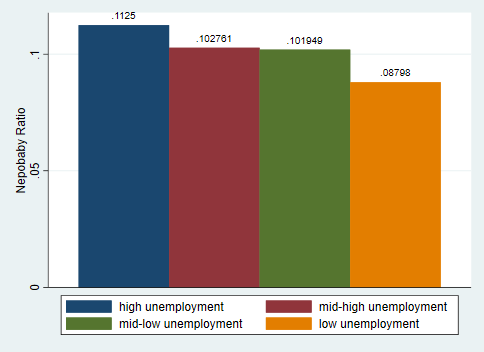
\includegraphics[width=0.65\linewidth]{neporatio.hirecategory.png}
    \caption{Ratios of Nepotism Hiring by Unemployment Level Hire Category}
    \label{fig:enter-label}
\end{figure}

We also performed a sensitivity analysis to determine if that result held up to slight changes in the way that a respondent's job length was defined. Because of the imprecise nature of the way that hire month was defined, and therefore the uncertainty in the assigned unemployment rate, as mentioned in Section \ref{sec:data}, we test whether variations of this definition impact the result. Because the employment length variable is only measured at the years level, while unemployment rate is measured at the months level, the assigned unemployment rate for each respondent is not exact. So, to test whether the result is sensitive to this measurement error, we run the same chi-square analysis, testing the association between nepotism status and unemployment level at hiring, using unemployment rates that are shifted back three months, shifted back six months, pushed forward three months, and pushed forward six months. Each of the four tests resulted a in a p-value greater than 0.05, providing evidence for the result of the original chi-square analysis, and providing evidence that the measurement error in estimating hire month is not a notable cause for concern in the validity of this result.

\begin{figure}
    \centering
    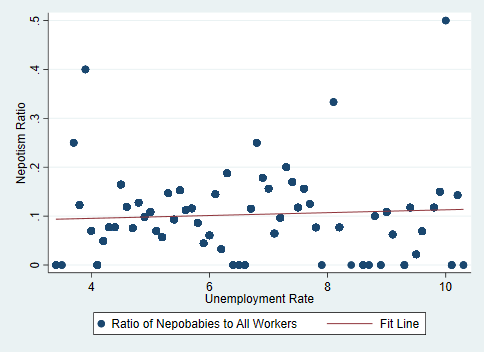
\includegraphics[width=0.65\linewidth]{neporatio.urate.correlation.png}
    \caption{Nepotism Ratio vs. Unemployment Rate}
    \label{fig:enter-label}
\end{figure}

Additionally, we use a logistic regression model to test the hypothesis. The response variable is the binary nepotism status variable, and the predictor variable is the continuous unemployment rate variable. Similar to the chi-square analysis, we do not find enough evidence to reject the null hypothesis that the unemployment rate that one is hired under is a strong predictor of nepotism status. The p-value for the likelihood ratio chi-square statistic, i.e. an indicator of whether the unemployment ratio is a significant predictor of variation in nepotism status, is 0.418, which strengthens the results from the chi-square analysis and provides more evidence that the unemployment rate does not strongly explain variation in nepotism rates. Additionally, the coefficient associated with the unemployment rate is 1.032, meaning that a one percentage point increase in the unemployment rate will result in a 3.2 percent higher likelihood that one is a nepobaby. However, the p-value associated with this coefficient is 0.415, so this effect is not statistically significant. The logistic regression model provides no evidence that the null hypothesis can be rejected, and therefore supports the claim that the unemployment rate at the time of hiring does not significantly affect the nepotism status of a new-hire. This weak, if not nonexistent relationship can be seen in Figure 2, where a loosely dispersed set of nepotism ratios show no clear effect from the unemployment rate.



The last test we used to examine the association between labor market competition and nepotism status is a test of correlation. We represented the level of nepotism as a ratio of nepobabies to all workers during each unemployment rate at 0.1 percentage point intervals as calculated by the FRED. This correlation had a coefficient of 0.0979, marking some weak relationship between the two. Unlike the results from the chi-square analysis and the logistic regression, the p-value for this test was very low and statistically significant at a 99.9 percent significance level, suggesting that there is some relationship between the two variables. While there might be some statistically significant relationship, it is clear that unemployment rate at time of hire does not explain the variation in nepotism status.

For the second part of our analysis, we looked at the gender dynamics of nepotistic parent-child relationships and the demographics of nepobabies. As expected, we find that children are much more likely to find themselves in a nepotistic relationship with their parent of the same gender than they are for the parent of the opposite gender. Nepotistic mothers, of which there were 118 when excluding mothers who had the same industry as the respondent’s father, were much more likely to have their daughters in the same industry than their sons. 



Of the 113 nepotistic daughter-parent relationships, 74 percent were mothers and only 26 percent were fathers, excluding cases where a daughter was in the same industry as both parents. This highly gendered relationship holds true for the 150 nepotistic son-parent relationships (when excluding fathers who had the same industry as the respondent’s mother). Of the nepotistic son-parent relationships, 77 percent were fathers and only 33 percent were mothers. It is then no surprise that running a chi-square analysis testing the association between nepotistic parent sex and nepotistic child sex is statistically significant at a 99.9 percent significance level. This dramatic relationship can be seen in the grouped-bar chart shown in Figure 3. While labor market gender dynamics, i.e. the gendered and sex-stereotyped roles that exist ubiquitously in the labor market, make this relationship no surprise, we see opportunity for further study on this relationship. It is unclear whether or not fathers feel more comfortable or are in better positions to support their children in finding jobs, or vice versa.

\begin{figure}
    \centering
    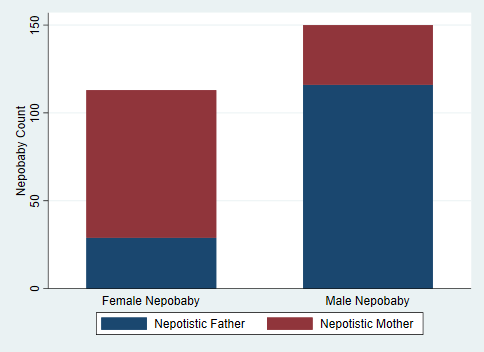
\includegraphics[width=0.65\linewidth]{nepoparent.sexcounts.png}
    \caption{Frequencies of Nepobaby Sex and Nepotistic Parent Sex}
    \label{fig:enter-label}
\end{figure}

We then examined different demographics to compare nepobabies to the rest of the sample. First, we tested how race differs between the nepobabies and non-nepobabies within our sample. A chi-square test measuring the association between race and nepotism status yields no significant result. We ran similar chi-square analyses and found no statistically significant association between nepobaby status and the following demographics: gender, education level, and (self-reported) class. We likewise tested the average number of years of education of nepobabies and non-nepobabies using a two-sample t-test and found no significant result. The difference in means for average income was not significant at conventional levels (p = 0.0866), but provides some weak evidence that nepobabies may have higher salaries than their counterparts that were not hired as products of nepotism.

We also examined how nepobabies may behave or be treated differently than their counterparts in the workplace. Using a variable that marks the likelihood that a respondent thinks they will lose their job, we found that nepobabies feel more secure in their workplaces. While only 65 percent of all workers in our sample said they think it is not likely that they will lose their job, 73 percent of nepobabies believe that it is unlikely they will lose their job. From the chi-square test we conducted, we can say with 95 percent confidence that there is a statistically significant difference between the proportion of nepobabies who feel more confident in the safety of their employment status than the rest of the sample. This provides further evidence of the benefit that nepobabies receive by taking advantage of their parental connections to find and maintain employment. We found no statistically significant difference between nepobabies and non-nepobabies in terms of another work related feature in the data set, hours worked per week. From the two-sample t-tests we ran, nepobabies did not work a significantly different amount of hours each week.

From the statistical tests we performed, we have no evidence that there is a significant association between the level of unemployment (representing the competitiveness of the labor market) and the rate of nepotism among young adults joining the labor market. Our hypothesis that we sought to test is that when labor markets are more competitive, young adults will be compelled to take advantage of their resources, specifically their parents, and create nepotistic relationships in order to find employment. From the results of the chi-square analysis, the robustness check, and the logistic regression model, we cannot reject the null hypothesis; the level of labor market competition does not drive differences in the rate of nepotistic relationships between young adults and their parents. We also find that nepobabies are more likely to feel safe in their job and are more likely to follow their same-sex parent into the same industry, providing us with some information on who nepobabies are and how being a product of nepotism has altered their working experience. It is also important to note the weak evidence that nepobabies make more money than non-nepobabies, and we recommend that in future studies with larger sample sizes that this relationship be studied more closely.


\section{Discussion}
\label{sec:discussion}
The results from our analysis ultimately provide little evidence for our research hypothesis. It is important to recognize the factors that limit the strength of our results and give opportunity for others to build on our findings. First, there are some limitations in our data sets that could be addressed in future research. The FRED unemployment rate data set that we used to evaluate were national averages of the U.S. unemployment rate. Of course, that average does not necessarily pertain to each observation/individual. Future work could use state or county averages to better estimate the effects of labor market competition on rates of nepotism, given that the locale where a respondent was hired is collected in the survey.. Additionally, the variable we used to estimate the month at which a GSS respondent was hired was not perfectly accurate. Respondents could only answer that they had been employed at their current job for three months, nine months, or whole years starting at 1 and counting up. This means that the month of hire we assigned for each respondent may not be exact. More precise measures of the amount of time someone has held their job could allow for more accurate analysis. Lastly, there are significant limitations of how a nepobaby is defined. We defined nepobabies as having at least one parent in the same industry as the respondent, with the industry matching based on the 2007 NAICS codes. However, just because someone is in the same industry as a parent does not mean that they were on the receiving end of nepotism in finding employment. Additionally, just because someone is not in the same industry as one of their parents does not mean that they were not on the receiving end of nepotism. For example, a young adult may have used their parents connections in their desired industry to create nepotistic relationships to find employment, likely demonstrating that they went to further lengths to find employment. Our data set does not contain information on this type of nepotism or on the amount of effort a person put into using their resources for finding employment. Additional analysis would benefit from obtaining information on these other forms of nepotism and on how respondents used their resources to gain employment so that this could be analyzed over the business cycle.

We also encourage policymakers and administrators in secondary and higher education to examine these results and consider their implications. While we only found a few areas where nepobabies had significantly different characteristics than the sample at large, this analysis was limited by the characteristics noted in the GSS data set. However, it can be certain that such nepotistic relationships and their support in helping young adults find jobs gives an advantage to those who have living, working parents and to those who have good relationships with their parents. The use of such nepotistic relationships inherently creates an inequality between young adults who can use their parents’ status to gain employment and young adults who do not have that resource. Policymakers and administrators of educational institutions, especially those focused on creating equity, may find these results troubling. Support systems for those who cannot access these resources may be put into place to give those who lack such resources an equal opportunity to find employment.


\section{Conclusion}
\label{sec:conclusion}


We do not find strong evidence that labor market competition levels have a significant impact on the rate of nepotistic relationship formation that helps young adults to find employment as they enter the labor market, and we posit that this is due to strong forces encouraging nepotistic relationships that are omnipresent. Nepotistic relationships, where a young adult works within the same industries as at least one of their parents, do not have a significantly greater likelihood of forming during poor economic times. By matching respondents’ industries to their parents’ industries, the respondents classified as nepobabies were seen frequently but without any significant variation across the business cycle. We provide evidence for the theory that nepotistic relationships are common and consistently occurring, such that economic conditions have little to no significant impact on the frequency of the relationships being formed. 
We use two data sets, both pertaining to people and conditions within the United States. The GSS offers data on respondents' answers to questions including their demographic information, employment status, and questions regarding family relationships. The FRED data set includes monthly unemployment rates from 1960 to 2022. These data sets allow for a preliminary evaluation of young adults, specifically those in nepotistic relationships, gaining employment during different economic conditions.
Measuring the times in which someone was hired and matching this time to the monthly unemployment rate indicates if nepotism was used under more competitive labor market conditions. As noted in the literature review, poor economic conditions result in labor market entrants experiencing difficulty entering the workforce. By gaining employment through relatives, specifically parents, young professionals create nepotistic relationships as a form of using resources to find employment. Through economic cycles, nepobabies are found to be nearly evenly dispersed, suggesting that nepotistic relationships and the motivations that create them are powerful and unlikely to be swayed by labor market conditions. 



\newpage
\singlespacing
\setlength\bibsep{1pt}

\bibliographystyle{apalike}
\bibliography{nepobabiesreferences.bib}

\newpage
\appendix
\section{Appendix}
\label{sec:appendix}

\newcommand{\hrefunderline}[2]{\href{#1}{\textcolor{darkblue}{\uline{#2}}}}

\definecolor{darkblue}{rgb}{0.0, 0.0, 0.5}

\hypersetup{
    linkcolor=darkblue,    % Color of internal links
    citecolor=darkblue,    % Color of citations
    filecolor=darkblue,    % Color of file links
    urlcolor=darkblue      % Color of external links
}

The data files, code and output used for analysis, and documentation for this project can be found in the nepobabies \hrefunderline{https://github.com/ecn310/course-project-nepobabies}{GitHub repository}. All information and files needed to reproduce these results can be found in a 
\hrefunderline{https://github.com/ecn310/course-project-nepobabies/blob/main/Final\%20Report/ReproducibilityPackage.md}{reproducibility package}
in this repository. All figures can be found in the 
\hrefunderline{https://github.com/ecn310/course-project-nepobabies/tree/main/Final\%20Report/figures}{figures} 
folder in the repository. The code used to complete the analysis is in a file titled \hrefunderline{https://github.com/ecn310/course-project-nepobabies/blob/main/DoFiles/nepobabies.do}{nepobabies.do}. The results can be viewed in a file titled \hrefunderline{https://github.com/ecn310/course-project-nepobabies/blob/main/DoFiles/nepobabies.log}{nepobabies.log}.

In \hrefunderline{https://sumailsyr-my.sharepoint.com/personal/rhrabino_syr_edu/_layouts/15/onedrive.aspx?id=\%2Fpersonal\%2Frhrabino\%5Fsyr\%5Fedu\%2FDocuments\%2FECN\%20310\%20Project&FolderCTID=0x012000B87F490D5FFF3342AC97956897C98D3E&view=0}{OneDrive}, one can access the original, uncleaned GSS dataset, which contains all GSS observations from 1972-2022 and is titled "gss7222\_r1.dta." Likewise, the original GSS data can be obtained directly from the source from the \hrefunderline{https://gss.norc.org/get-the-data/stata}{GSS} website. The cleaned dataset, which removed variables of no interest, is in OneDrive and titled "GSSclean\_noRDs.dta."



\end{document}